\section{Additional Results}\label{app:figures}

This appendix reports the participation profiles under the instrument eliminations of Section~\ref{sec:results_elim} and the reforms of the upper replacement rates of the PIA formula.

\paragraph{Participation under the instrument eliminations.} \autoref{fig:elim_lfpr} shows the participation profiles of the whole cohort under the five eliminations of \autoref{tab:elim}, and \autoref{fig:elim_lfpr_health} shows them by health status. Eliminating Social Security lowers participation before age 50, by up to about 4 percentage points in the aggregate and by up to about 6 and 9 points in poor health and with a disability, and raises it afterward in every health state: from age 50 for individuals with a disability, from the early 50s for those in poor health, and from the mid-50s for those in good health. Eliminating DI leaves participation unchanged before age 50 and raises it afterward in every health state, most for individuals with a disability, for whom DI is the main pathway out of the labor force. Full Medicare coverage, the full savings subsidy, and the abolition of the income tax lower aggregate participation at older ages.
% Derived: figures/frot_weld1.tex, frot_weld1_1.tex, frot_weld1_2.tex (D1 minus Model, ages 40-49): aggregate down to -3.7 pp (age 49), poor health -6.4 (48), disability -9.5 (45).

\begin{figure}[!htbp]
\centering
\caption{Participation under the Elimination of Policy Instruments}\label{fig:elim_lfpr}
\vspace{0.5em}
% Panels copied verbatim from the FROT project (figures/abdou/frot_weld1.tex, frot_weld2.tex), arranged as in FROT 2025_sub/12_app_quant.tex.
% AUTHORS: reform and elimination results are from the May 2025 simulation; fit figures are the 2026 corrected re-simulation. Rerun reforms on the corrected code before submission.
\begin{tabular}{@{}c@{\hspace{1em}}c@{}}
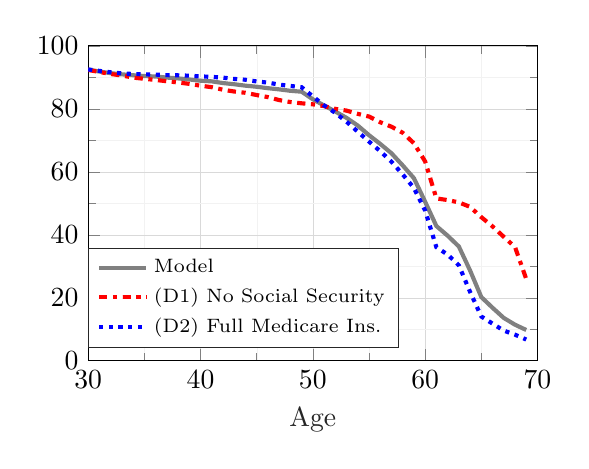
\begin{tikzpicture}
\begin{axis}[%
width=5.706cm,
height=4cm,
at={(0cm,0cm)},
scale only axis,
xmin=30,
xmax=70,
xlabel style={font=\color{white!15!black}},
xlabel={Age},
ymin=-0,
ymax=0100,
ylabel style={font=\color{white!15!black}},
ylabel={},
axis background/.style={fill=white},
%title style={font=\bfseries},
title={},
legend style={at={(axis cs:30,20)}, anchor=west, legend cell align=left, align=left, draw=white!15!black, font=\scriptsize},
grid=both,
grid style={line width=0.2pt, draw=gray!30},
minor grid style={line width=0.1pt, draw=gray!10},
minor tick num=1
]
% Back line (Overall) - full
\addplot [color=gray, line width=1.5pt]
  table[row sep=crcr]{%
30		92.457143	\\
31		91.828571	\\
32		91.314286	\\
33		90.942857	\\
34		90.657143	\\
35		90.4	\\
36		90.257143	\\
37		89.914286	\\
38		89.657143	\\
39		89.314286	\\
40		88.914286	\\
41		88.714286	\\
42		88.171429	\\
43		87.8	\\
44		87.342857	\\
45		87	\\
46		86.542857	\\
47		86.171429	\\
48		85.714286	\\
49		85.428571	\\
50		83.028571	\\
51		81.057143	\\
52		79.142857	\\
53		77.114286	\\
54		74.685714	\\
55		71.628571	\\
56		68.857143	\\
57		65.885714	\\
58		62.028571	\\
59		57.971429	\\
60		50.485714	\\
61		42.771429	\\
62		39.714286	\\
63		36.285714	\\
64		28.657143	\\
65		20.228571	\\
66		16.828571	\\
67		13.6	\\
68		11.457143	\\
69		9.771429	\\
};
\addlegendentry{Model}
% Blue line (Good health) - dotted
\addplot [color=red, line width=1.5pt, dashdotted]
  table[row sep=crcr]{%
30	92.342857	\\
31	91.685714	\\
32	91.057143	\\
33	90.571429	\\
34	89.914286	\\
35	89.514286	\\
36	89.171429	\\
37	88.742857	\\
38	88.371429	\\
39	87.914286	\\
40	87.342857	\\
41	86.857143	\\
42	86.057143	\\
43	85.485714	\\
44	85.085714	\\
45	84.371429	\\
46	83.714286	\\
47	82.771429	\\
48	82.142857	\\
49	81.742857	\\
50	81.428571	\\
51	80.857143	\\
52	79.971429	\\
53	79.428571	\\
54	78.4	\\
55	77.542857	\\
56	75.742857	\\
57	74.314286	\\
58	72.4	\\
59	69.057143	\\
60	63.285714	\\
61	51.542857	\\
62	51.028571	\\
63	50.285714	\\
64	48.857143	\\
65	45.6	\\
66	42.657143	\\
67	39.342857	\\
68	36.114286	\\
69	25.971429	\\
};
\addlegendentry{(D1) No Social Security}

% Red line (Poor health) - dash-dotted
\addplot [color=blue, line width=1.5pt, dotted]
  table[row sep=crcr]{%
30	92.485714	\\
31	92.028571	\\
32	91.6	\\
33	91.228571	\\
34	91.057143	\\
35	90.942857	\\
36	90.857143	\\
37	90.685714	\\
38	90.628571	\\
39	90.514286	\\
40	90.285714	\\
41	90.142857	\\
42	89.885714	\\
43	89.485714	\\
44	89.228571	\\
45	88.685714	\\
46	88.314286	\\
47	87.685714	\\
48	87.257143	\\
49	86.857143	\\
50	83.942857	\\
51	81.085714	\\
52	78.714286	\\
53	75.914286	\\
54	72.742857	\\
55	69.6	\\
56	66.542857	\\
57	63.2	\\
58	59.171429	\\
59	54.857143	\\
60	47.685714	\\
61	36.057143	\\
62	33.714286	\\
63	30.314286	\\
64	21.857143	\\
65	14.057143	\\
66	11.8	\\
67	9.571429	\\
68	8.285714	\\
69	6.742857	\\
};
\addlegendentry{(D2) Full Medicare Ins.}

% Green line (Disabled) - dashed
% \addplot [color=green, line width=1.5pt, dashed]
%   table[row sep=crcr]{%
% 30	92.6	\\
% 31	92.2	\\
% 32	91.7714286	\\
% 33	91.4285714	\\
% 34	91.2571429	\\
% 35	91.1142857	\\
% 36	91.0571429	\\
% 37	90.8857143	\\
% 38	90.8285714	\\
% 39	90.7142857	\\
% 40	90.4571429	\\
% 41	90.2857143	\\
% 42	90.0285714	\\
% 43	89.6571429	\\
% 44	89.3142857	\\
% 45	88.7714286	\\
% 46	88.2857143	\\
% 47	87.6571429	\\
% 48	87.1714286	\\
% 49	86.6285714	\\
% 50	83.7142857	\\
% 51	80.8285714	\\
% 52	78.5428571	\\
% 53	75.9142857	\\
% 54	72.8857143	\\
% 55	69.7428571	\\
% 56	66.6285714	\\
% 57	63.1428571	\\
% 58	59.0857143	\\
% 59	54.7714286	\\
% 60	47.2571429	\\
% 61	35.0571429	\\
% 62	32.8285714	\\
% 63	29.5714286	\\
% 64	21.0571429	\\
% 65	5.5714286	\\
% 66	3.1428571	\\
% 67	2.0285714	\\
% 68	1.3428571	\\
% 69	0.7142857	\\
% };
% \addlegendentry{Medicare B Reform Full}
\end{axis}
\end{tikzpicture} & 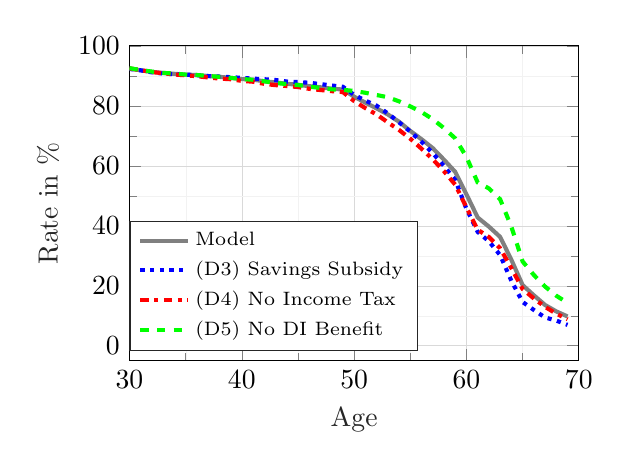
\begin{tikzpicture}
\begin{axis}[%
width=5.706cm,
height=4cm,
at={(0cm,0cm)},
scale only axis,
xmin=30,
xmax=70,
xlabel style={font=\color{white!15!black}},
xlabel={Age},
ymin=-5,
ytick={0,20,...,100},
ymax=0100,
ylabel style={font=\color{white!15!black}},
ylabel={Rate in \%},
axis background/.style={fill=white},
%title style={font=\bfseries},
title={},
legend style={at={(axis cs:30,20)}, anchor=west, legend cell align=left, align=left, draw=white!15!black, font=\scriptsize},
grid=both,
grid style={line width=0.2pt, draw=gray!30},
minor grid style={line width=0.1pt, draw=gray!10},
minor tick num=1
]
% Back line (Overall) - full
\addplot [color=gray, line width=1.5pt]
  table[row sep=crcr]{%
30		92.457143	\\
31		91.828571	\\
32		91.314286	\\
33		90.942857	\\
34		90.657143	\\
35		90.4	\\
36		90.257143	\\
37		89.914286	\\
38		89.657143	\\
39		89.314286	\\
40		88.914286	\\
41		88.714286	\\
42		88.171429	\\
43		87.8	\\
44		87.342857	\\
45		87	\\
46		86.542857	\\
47		86.171429	\\
48		85.714286	\\
49		85.428571	\\
50		83.028571	\\
51		81.057143	\\
52		79.142857	\\
53		77.114286	\\
54		74.685714	\\
55		71.628571	\\
56		68.857143	\\
57		65.885714	\\
58		62.028571	\\
59		57.971429	\\
60		50.485714	\\
61		42.771429	\\
62		39.714286	\\
63		36.285714	\\
64		28.657143	\\
65		20.228571	\\
66		16.828571	\\
67		13.6	\\
68		11.457143	\\
69		9.771429	\\
};
\addlegendentry{Model}


% Red line (Poor health) - dash-dotted
\addplot [color=blue, line width=1.5pt, dotted]
  table[row sep=crcr]{%
30	92.285714	\\
31	91.828571	\\
32	91.142857	\\
33	90.742857	\\
34	90.542857	\\
35	90.4	\\
36	90.2	\\
37	89.914286	\\
38	89.742857	\\
39	89.542857	\\
40	89.314286	\\
41	89.057143	\\
42	88.857143	\\
43	88.6	\\
44	88.085714	\\
45	87.914286	\\
46	87.685714	\\
47	87.228571	\\
48	86.771429	\\
49	86.342857	\\
50	83.657143	\\
51	81.742857	\\
52	80.028571	\\
53	77.457143	\\
54	74.485714	\\
55	71.4	\\
56	68	\\
57	64.228571	\\
58	59.942857	\\
59	55.285714	\\
60	45.657143	\\
61	37.971429	\\
62	34.828571	\\
63	30.228571	\\
64	21.657143	\\
65	14.6	\\
66	11.942857	\\
67	9.428571	\\
68	8.4	\\
69	6.971429	\\
};
\addlegendentry{(D3) Savings Subsidy}
% Blue line (Good health) - dotted
\addplot [color=red, line width=1.5pt, dashdotted]
  table[row sep=crcr]{%
30	92.485714	\\
31	91.857143	\\
32	91.257143	\\
33	90.857143	\\
34	90.428571	\\
35	90.171429	\\
36	89.857143	\\
37	89.457143	\\
38	89.085714	\\
39	88.857143	\\
40	88.314286	\\
41	88.028571	\\
42	87.314286	\\
43	86.885714	\\
44	86.6	\\
45	86.257143	\\
46	85.657143	\\
47	85.257143	\\
48	84.885714	\\
49	84.571429	\\
50	81.571429	\\
51	79.228571	\\
52	77.114286	\\
53	74.485714	\\
54	71.942857	\\
55	69.028571	\\
56	65.685714	\\
57	62.171429	\\
58	58.171429	\\
59	53.714286	\\
60	46.114286	\\
61	38.685714	\\
62	36.257143	\\
63	32.514286	\\
64	25.885714	\\
65	18.914286	\\
66	15.771429	\\
67	12.971429	\\
68	10.685714	\\
69	8.857143	\\
};
\addlegendentry{(D4) No Income Tax}


% Green line (Disabled) - dashed
\addplot [color=green, line width=1.5pt, dashed]
  table[row sep=crcr]{%
30	92.542857	\\
31	91.914286	\\
32	91.4	\\
33	90.971429	\\
34	90.742857	\\
35	90.4	\\
36	90.257143	\\
37	89.942857	\\
38	89.657143	\\
39	89.314286	\\
40	88.942857	\\
41	88.685714	\\
42	88.171429	\\
43	87.6	\\
44	87.257143	\\
45	86.942857	\\
46	86.371429	\\
47	85.971429	\\
48	85.485714	\\
49	85.342857	\\
50	84.942857	\\
51	84.342857	\\
52	83.6	\\
53	82.857143	\\
54	81.485714	\\
55	79.8	\\
56	77.914286	\\
57	75.542857	\\
58	72.571429	\\
59	69.142857	\\
60	62.942857	\\
61	54.428571	\\
62	52.457143	\\
63	48.828571	\\
64	39.685714	\\
65	28.114286	\\
66	23.6	\\
67	19.742857	\\
68	16.685714	\\
69	14.285714	\\
};
\addlegendentry{(D5) No DI Benefit}
\end{axis}
\end{tikzpicture}
\end{tabular}
\tabnotes{\textit{Notes:} Labor force participation rate (percent) by age, simulated from the estimated model (Model) and from counterfactual economies that eliminate one policy instrument. Left panel: the \textit{No Social Security} experiment (D1) sets Social Security benefits to zero; the \textit{Full Medicare Insurance} experiment (D2) sets out-of-pocket medical expenses after age 65 to zero for participants and nonparticipants. Right panel: the \textit{Full Savings Subsidy} experiment (D3) sets the net return on assets equal to the pretax return; the \textit{No Income Tax} experiment (D4) sets the income tax to zero; the \textit{No Disability Benefit} experiment (D5) sets disability benefits to zero. The \textit{No Social Security} experiment produces the largest increase in participation, followed by the \textit{No Disability Benefit} experiment. Welfare effects are in \autoref{tab:elim}.}
\end{figure}

\paragraph{Upper replacement rates.} \autoref{tab:generosity_app} reports reforms that raise the second replacement rate of the PIA formula from 0.32 to 0.352 (P2.0--P2.9) and then the third from 0.15 to 0.165 (P3.0--P3.9), in steps of 1 percent of the initial rate. All of them keep the first rate at 0.99, the value under P1.9, so each row, MVPF included, reports the total effect relative to the status quo, and the effect of the upper rates is the difference between a row and P1.9 in \autoref{tab:generosity}. Across P2.0--P2.9, the cumulative MVPF falls from 0.56 to 0.29: WTP rises from 0.83 to 0.95 percent, while the net cost more than doubles, from 0.57 to 1.27 percent. Relative to P1.9, P2.9 adds 0.15 percent to WTP and 0.83 percent to the net cost. Raising the third rate changes neither WTP nor the net cost by more than a few hundredths of a percentage point, within the precision of the simulations, and the MVPF stays at 0.29--0.30. Participation at 30--49 rises by 0.24 to 0.28 points, and participation at 62--64 and 65--69 falls by 0.83 to 2.41 points, more than under any bottom-bracket reform. P3.9 and L9 set the same three rates, (0.99, 0.352, 0.165), and their rows coincide.

\begin{table}[!htbp]
\centering
\caption{Reforms of the Upper Replacement Rates}\label{tab:generosity_app}
\footnotesize
\setlength{\tabcolsep}{4.5pt}
% Source: FROT tables/welfare_progressivity_mvpfv7.tex, rows P2 and P3.
% AUTHORS: reform and elimination results are from the May 2025 simulation; fit figures are the 2026 corrected re-simulation. Rerun reforms on the corrected code before submission.
% Generated by gen_tables.py from FROT tables/welfare_progressivity_mvpfv7.tex (rows P2, P3).
% Source numbers: May 2025 simulation of the estimated model (FROT 2025 submission). Do not edit numbers by hand.
\begin{tabular}{@{}l l c c c c c c c c@{}}
\toprule
 & & \multicolumn{2}{c}{Welfare} & \multicolumn{3}{c}{Fiscal cost (\% change)} & \multicolumn{3}{c}{$\Delta$ Participation (pp)} \\
\cmidrule(lr){3-4}\cmidrule(lr){5-7}\cmidrule(lr){8-10}
 & PIA rates & MVPF & WTP (\%) & Net & Direct & Indirect & 30--49 & 62--64 & 65--69 \\
\midrule
\multicolumn{10}{@{}l}{\textit{A. Raising the second PIA rate (first rate at 0.99)}} \\
(P2.0) & (0.99, 0.3232, 0.15) & 0.56 & 0.83 & 0.57 & 4.75 & $-$0.07 & 0.25 & $-$1.10 & $-$0.83 \\
(P2.1) & (0.99, 0.3264, 0.15) & 0.50 & 0.86 & 0.67 & 5.28 & $-$0.05 & 0.24 & $-$1.29 & $-$1.03 \\
(P2.2) & (0.99, 0.3296, 0.15) & 0.49 & 0.88 & 0.70 & 5.99 & $-$0.11 & 0.25 & $-$1.05 & $-$1.01 \\
(P2.3) & (0.99, 0.3328, 0.15) & 0.44 & 0.90 & 0.78 & 6.56 & $-$0.10 & 0.24 & $-$1.37 & $-$1.15 \\
(P2.4) & (0.99, 0.336, 0.15) & 0.38 & 0.92 & 0.93 & 7.21 & $-$0.05 & 0.24 & $-$1.60 & $-$1.63 \\
(P2.5) & (0.99, 0.3392, 0.15) & 0.37 & 0.93 & 0.98 & 7.95 & $-$0.10 & 0.27 & $-$1.63 & $-$1.58 \\
(P2.6) & (0.99, 0.3424, 0.15) & 0.36 & 0.95 & 1.03 & 8.46 & $-$0.11 & 0.28 & $-$1.47 & $-$1.68 \\
(P2.7) & (0.99, 0.3456, 0.15) & 0.33 & 0.94 & 1.11 & 8.99 & $-$0.10 & 0.27 & $-$1.74 & $-$1.99 \\
(P2.8) & (0.99, 0.3488, 0.15) & 0.31 & 0.95 & 1.19 & 9.49 & $-$0.10 & 0.28 & $-$2.29 & $-$2.10 \\
(P2.9) & (0.99, 0.352, 0.15) & 0.29 & 0.95 & 1.27 & 9.97 & $-$0.09 & 0.28 & $-$2.26 & $-$2.05 \\
\addlinespace
\multicolumn{10}{@{}l}{\textit{B. Raising the third PIA rate (first two rates at 0.99 and 0.352)}} \\
(P3.0) & (0.99, 0.352, 0.1515) & 0.29 & 0.95 & 1.26 & 10.04 & $-$0.10 & 0.28 & $-$2.22 & $-$2.05 \\
(P3.1) & (0.99, 0.352, 0.153) & 0.29 & 0.96 & 1.27 & 10.13 & $-$0.10 & 0.28 & $-$2.30 & $-$2.07 \\
(P3.2) & (0.99, 0.352, 0.1545) & 0.29 & 0.96 & 1.28 & 10.19 & $-$0.10 & 0.28 & $-$2.30 & $-$2.07 \\
(P3.3) & (0.99, 0.352, 0.156) & 0.29 & 0.96 & 1.26 & 10.26 & $-$0.13 & 0.28 & $-$2.25 & $-$2.03 \\
(P3.4) & (0.99, 0.352, 0.1575) & 0.29 & 0.96 & 1.27 & 10.34 & $-$0.13 & 0.28 & $-$2.23 & $-$2.03 \\
(P3.5) & (0.99, 0.352, 0.159) & 0.29 & 0.97 & 1.29 & 10.41 & $-$0.12 & 0.28 & $-$2.41 & $-$2.02 \\
(P3.6) & (0.99, 0.352, 0.1605) & 0.29 & 0.97 & 1.27 & 10.48 & $-$0.14 & 0.28 & $-$2.39 & $-$2.02 \\
(P3.7) & (0.99, 0.352, 0.162) & 0.30 & 0.97 & 1.27 & 10.55 & $-$0.15 & 0.28 & $-$2.39 & $-$2.02 \\
(P3.8) & (0.99, 0.352, 0.1635) & 0.30 & 0.97 & 1.25 & 10.63 & $-$0.18 & 0.28 & $-$2.37 & $-$2.01 \\
(P3.9) & (0.99, 0.352, 0.165) & 0.30 & 0.98 & 1.24 & 10.70 & $-$0.20 & 0.28 & $-$2.37 & $-$1.99 \\
\bottomrule
\end{tabular}

\tabnotes{\textit{Notes:} Each row reports the outcomes of simulating the estimated model for the cohort under the reform, announced before age 30 and in force over the life cycle, with prices held fixed (partial equilibrium). The second column gives the three replacement rates of the PIA formula; the status quo is (0.90, 0.32, 0.15). P2.0--P2.9 raise the second rate in steps of 0.32 percentage points with the first rate at 0.99; P3.0--P3.9 raise the third rate in steps of 0.15 percentage points with the first two rates at 0.99 and 0.352. Every row includes the increase of the first rate to 0.99 (P1.9 in \autoref{tab:generosity}) and reports the change from the status quo. WTP: ex ante consumption-equivalent welfare change at age 30, in percent. Direct: percentage change in the present value of Social Security retirement benefits. Indirect: percentage change in the present value of all other taxes and transfers (DI benefits and consumption-floor transfers, net of income- and payroll-tax revenue). Net: percentage change in the present value of net government spending. Present values are per capita and discounted to age 62 (Section~\ref{sec:fw_fiscal}); because the three fiscal columns have different bases, Net is not the sum of Direct and Indirect. MVPF: WTP valued with the present value of per capita baseline consumption from age 62, divided by the dollar change in net government spending (equation~\eqref{eq:mvpf}). $\Delta$ Participation: change in the labor force participation rate at the indicated ages, in percentage points. Abbreviations: AIME, average indexed monthly earnings; DI, disability insurance; PIA, primary insurance amount.}
\end{table}

\begin{figure}[!htbp]
\centering
\caption{Participation under the Elimination of Policy Instruments, by Health Status}\label{fig:elim_lfpr_health}
\vspace{0.5em}
% Panels copied verbatim from the FROT project (figures/abdou/frot_weld{1,2}_{0,1,2}.tex), arranged as in FROT 2025_sub/12_app_quant.tex; scaled to 0.9 to fit the page.
% AUTHORS: reform and elimination results are from the May 2025 simulation; fit figures are the 2026 corrected re-simulation. Rerun reforms on the corrected code before submission.
\begin{tabular}{@{}c@{\hspace{1em}}c@{}}
\multicolumn{2}{c}{\small (A) Good Health}\\[0.3ex]
\scalebox{0.9}{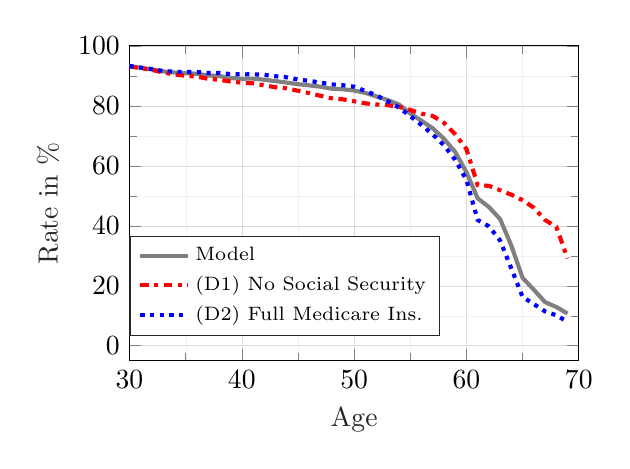
\begin{tikzpicture}
\begin{axis}[%
width=5.706cm,
height=4cm,
at={(0cm,0cm)},
scale only axis,
xmin=30,
xmax=70,
xlabel style={font=\color{white!15!black}},
xlabel={Age},
ymin=-5,
ytick={0,20,...,100},
ymax=0100,
ylabel style={font=\color{white!15!black}},
ylabel={Rate in \%},
axis background/.style={fill=white},
%title style={font=\bfseries},
title={},
legend style={at={(axis cs:30,20)}, anchor=west, legend cell align=left, align=left, draw=white!15!black, font=\scriptsize},
grid=both,
grid style={line width=0.2pt, draw=gray!30},
minor grid style={line width=0.1pt, draw=gray!10},
minor tick num=1
]
% Back line (Overall) - full
\addplot [color=gray, line width=1.5pt]
  table[row sep=crcr]{%
30	93.248945	\\
31	92.66386	\\
32	92.127404	\\
33	91.477788	\\
34	91.08492	\\
35	90.842714	\\
36	90.681332	\\
37	90.107527	\\
38	89.928947	\\
39	89.275723	\\
40	89.028213	\\
41	89.071383	\\
42	88.68104	\\
43	88.224061	\\
44	87.736151	\\
45	87.191157	\\
46	86.816406	\\
47	86.369637	\\
48	85.709527	\\
49	85.508219	\\
50	85.099111	\\
51	84.293015	\\
52	83.102493	\\
53	81.913775	\\
54	80.404686	\\
55	77.450628	\\
56	75	\\
57	72.50185	\\
58	68.992537	\\
59	64.610144	\\
60	57.880539	\\
61	49.142634	\\
62	46.258503	\\
63	42.21861	\\
64	33.333333	\\
65	22.642293	\\
66	18.667798	\\
67	14.554196	\\
68	12.927257	\\
69	10.749331	\\
};
\addlegendentry{Model}
% Blue line (Good health) - dotted
\addplot [color=red, line width=1.5pt, dashdotted]
  table[row sep=crcr]{%
30	93.128391	\\
31	92.543596	\\
32	91.947115	\\
33	91.145361	\\
34	90.420066	\\
35	90.051719	\\
36	89.734189	\\
37	89.001536	\\
38	88.662342	\\
39	88.094498	\\
40	87.711599	\\
41	87.492104	\\
42	86.810399	\\
43	86.187142	\\
44	85.814922	\\
45	85.013004	\\
46	84.244792	\\
47	83.333333	\\
48	82.511659	\\
49	82.15364	\\
50	81.510595	\\
51	80.817717	\\
52	80.436288	\\
53	80.196285	\\
54	79.659212	\\
55	78.599641	\\
56	77.405248	\\
57	76.609919	\\
58	74.328358	\\
59	70.514762	\\
60	65.587669	\\
61	53.585347	\\
62	53.301321	\\
63	51.848842	\\
64	50.347648	\\
65	48.525135	\\
66	46.033093	\\
67	41.914336	\\
68	39.658195	\\
69	29.125781	\\
};
\addlegendentry{(D1) No Social Security}

% Red line (Poor health) - dash-dotted
\addplot [color=blue, line width=1.5pt, dotted]
  table[row sep=crcr]{%
30	93.279084	\\
31	92.723993	\\
32	92.247596	\\
33	91.59867	\\
34	91.356905	\\
35	91.268634	\\
36	91.261839	\\
37	90.967742	\\
38	90.917516	\\
39	90.581287	\\
40	90.470219	\\
41	90.524321	\\
42	90.298034	\\
43	89.847231	\\
44	89.497278	\\
45	88.751625	\\
46	88.313802	\\
47	87.755776	\\
48	87.141905	\\
49	86.85005	\\
50	86.363636	\\
51	84.940375	\\
52	83.448753	\\
53	81.458114	\\
54	79.410721	\\
55	76.552962	\\
56	73.61516	\\
57	70.429312	\\
58	66.865672	\\
59	61.998486	\\
60	55.260116	\\
61	41.93297	\\
62	39.815926	\\
63	35.067046	\\
64	25.725971	\\
65	16.285833	\\
66	13.915995	\\
67	11.451049	\\
68	10.166521	\\
69	7.983943	\\
};
\addlegendentry{(D2) Full Medicare Ins.}

% % Green line (Disabled) - dashed
% \addplot [color=green, line width=1.5pt, dashed]
%   table[row sep=crcr]{%
% 30	88.42857143	\\
% 31	88.22857143	\\
% 32	87.85714286	\\
% 33	86.77142857	\\
% 34	86.57142857	\\
% 35	85.88571429	\\
% 36	85.51428571	\\
% 37	84.77142857	\\
% 38	84.25714286	\\
% 39	83.45714286	\\
% 40	82.62857143	\\
% 41	82.02857143	\\
% 42	81.51428571	\\
% 43	80.82857143	\\
% 44	79.97142857	\\
% 45	78.08571429	\\
% 46	77.54285714	\\
% 47	76	\\
% 48	74.71428571	\\
% 49	73.77142857	\\
% 50	72.02857143	\\
% 51	70.97142857	\\
% 52	68.62857143	\\
% 53	66.31428571	\\
% 54	63.85714286	\\
% 55	60.91428571	\\
% 56	57.57142857	\\
% 57	54.2	\\
% 58	51.11428571	\\
% 59	46.62857143	\\
% 60	40.71428571	\\
% 61	29.94285714	\\
% 62	27.68571429	\\
% 63	23.88571429	\\
% 64	17.48571429	\\
% 65	5.314285714	\\
% 66	3	\\
% 67	1.942857143	\\
% 68	1.257142857	\\
% 69	0.685714286	\\
% };
% \addlegendentry{Medicare B Reform Full}
\end{axis}
\end{tikzpicture}} & \scalebox{0.9}{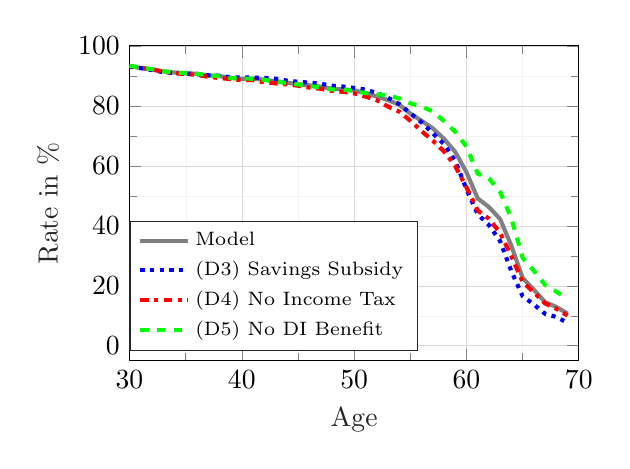
\begin{tikzpicture}
\begin{axis}[%
width=5.706cm,
height=4cm,
at={(0cm,0cm)},
scale only axis,
xmin=30,
xmax=70,
xlabel style={font=\color{white!15!black}},
xlabel={Age},
ymin=-5,
ytick={0,20,...,100},
ymax=0100,
ylabel style={font=\color{white!15!black}},
ylabel={Rate in \%},
axis background/.style={fill=white},
%title style={font=\bfseries},
title={},
legend style={at={(axis cs:30,20)}, anchor=west, legend cell align=left, align=left, draw=white!15!black, font=\scriptsize},
grid=both,
grid style={line width=0.2pt, draw=gray!30},
minor grid style={line width=0.1pt, draw=gray!10},
minor tick num=1
]
% Back line (Overall) - full
\addplot [color=gray, line width=1.5pt]
  table[row sep=crcr]{%
30	93.248945	\\
31	92.66386	\\
32	92.127404	\\
33	91.477788	\\
34	91.08492	\\
35	90.842714	\\
36	90.681332	\\
37	90.107527	\\
38	89.928947	\\
39	89.275723	\\
40	89.028213	\\
41	89.071383	\\
42	88.68104	\\
43	88.224061	\\
44	87.736151	\\
45	87.191157	\\
46	86.816406	\\
47	86.369637	\\
48	85.709527	\\
49	85.508219	\\
50	85.099111	\\
51	84.293015	\\
52	83.102493	\\
53	81.913775	\\
54	80.404686	\\
55	77.450628	\\
56	75	\\
57	72.50185	\\
58	68.992537	\\
59	64.610144	\\
60	57.880539	\\
61	49.142634	\\
62	46.258503	\\
63	42.21861	\\
64	33.333333	\\
65	22.642293	\\
66	18.667798	\\
67	14.554196	\\
68	12.927257	\\
69	10.749331	\\
};
\addlegendentry{Model}


% Red line (Poor health) - dash-dotted
\addplot [color=blue, line width=1.5pt, dotted]
  table[row sep=crcr]{%
30	93.068113	\\
31	92.543596	\\
32	91.917067	\\
33	91.205802	\\
34	90.903596	\\
35	90.751445	\\
36	90.55912	\\
37	90.168971	\\
38	90.021625	\\
39	89.524402	\\
40	89.404389	\\
41	89.418825	\\
42	89.28345	\\
43	89.05156	\\
44	88.408581	\\
45	88.003901	\\
46	87.727865	\\
47	87.359736	\\
48	86.708861	\\
49	86.413955	\\
50	85.95352	\\
51	85.417376	\\
52	84.279778	\\
53	82.719944	\\
54	80.617678	\\
55	77.522442	\\
56	74.489796	\\
57	70.873427	\\
58	67.201493	\\
59	61.619985	\\
60	52.2158	\\
61	43.842557	\\
62	40.256102	\\
63	34.863876	\\
64	24.867076	\\
65	16.535106	\\
66	13.788714	\\
67	10.664336	\\
68	9.596845	\\
69	7.671722	\\
};
\addlegendentry{(D3) Savings Subsidy}


% Blue line (Good health) - dotted
\addplot [color=red, line width=1.5pt, dashdotted]
  table[row sep=crcr]{%
30	93.279084	\\
31	92.66386	\\
32	92.097356	\\
33	91.387126	\\
34	90.873376	\\
35	90.568908	\\
36	90.314696	\\
37	89.677419	\\
38	89.280198	\\
39	88.902704	\\
40	88.526646	\\
41	88.566014	\\
42	87.824984	\\
43	87.492043	\\
44	87.159782	\\
45	86.703511	\\
46	86.067708	\\
47	85.676568	\\
48	84.976682	\\
49	84.669574	\\
50	84.142174	\\
51	83.100511	\\
52	81.890582	\\
53	79.775675	\\
54	78.097267	\\
55	75.044883	\\
56	71.574344	\\
57	68.393782	\\
58	64.776119	\\
59	59.91673	\\
60	52.83237	\\
61	45.089634	\\
62	42.336935	\\
63	37.667615	\\
64	29.856851	\\
65	21.354383	\\
66	17.776835	\\
67	14.117133	\\
68	12.357581	\\
69	10.080285	\\
};
\addlegendentry{(D4) No Income Tax}
% Green line (Disabled) - dashed
\addplot [color=green, line width=1.5pt, dashed]
  table[row sep=crcr]{%
30	93.339361	\\
31	92.723993	\\
32	92.217548	\\
33	91.508008	\\
34	91.175582	\\
35	90.842714	\\
36	90.681332	\\
37	90.138249	\\
38	89.928947	\\
39	89.275723	\\
40	89.059561	\\
41	89.039798	\\
42	88.649334	\\
43	88.0331	\\
44	87.64009	\\
45	87.126138	\\
46	86.653646	\\
47	86.138614	\\
48	85.443038	\\
49	85.441127	\\
50	84.92823	\\
51	84.258944	\\
52	83.864266	\\
53	83.42096	\\
54	82.499113	\\
55	80.825853	\\
56	79.737609	\\
57	78.164323	\\
58	74.88806	\\
59	71.347464	\\
60	66.396917	\\
61	57.404521	\\
62	55.782313	\\
63	51.279967	\\
64	42.494888	\\
65	29.372663	\\
66	24.989393	\\
67	20.323427	\\
68	18.054338	\\
69	15.566459	\\
};
\addlegendentry{(D5) No DI Benefit}
\end{axis}
\end{tikzpicture}} \\[0.4ex]
\multicolumn{2}{c}{\small (B) Poor Health}\\[0.3ex]
\scalebox{0.9}{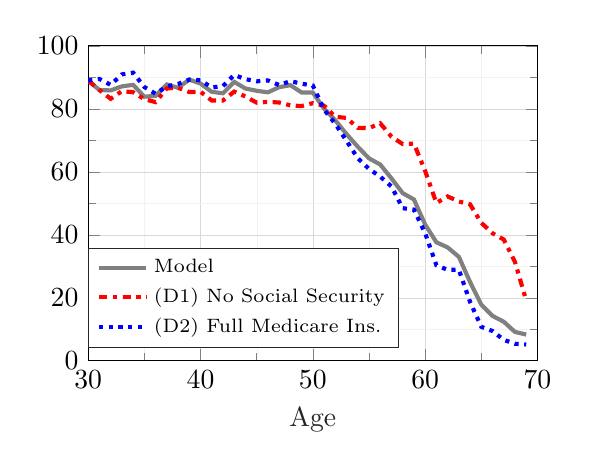
\begin{tikzpicture}
\begin{axis}[%
width=5.706cm,
height=4cm,
at={(0cm,0cm)},
scale only axis,
xmin=30,
xmax=70,
xlabel style={font=\color{white!15!black}},
xlabel={Age},
ymin=-0,
ymax=0100,
ylabel style={font=\color{white!15!black}},
ylabel={},
axis background/.style={fill=white},
%title style={font=\bfseries},
title={},
legend style={at={(axis cs:30,20)}, anchor=west, legend cell align=left, align=left, draw=white!15!black, font=\scriptsize},
grid=both,
grid style={line width=0.2pt, draw=gray!30},
minor grid style={line width=0.1pt, draw=gray!10},
minor tick num=1
]
% Back line (Overall) - full
\addplot [color=gray, line width=1.5pt]
  table[row sep=crcr]{%
30	88.970588	\\
31	85.964912	\\
32	85.840708	\\
33	87.121212	\\
34	87.596899	\\
35	83.846154	\\
36	84.10596	\\
37	87.730061	\\
38	86.666667	\\
39	89.265537	\\
40	88.020833	\\
41	85.388128	\\
42	84.931507	\\
43	88.546256	\\
44	86.440678	\\
45	85.714286	\\
46	85.227273	\\
47	86.851211	\\
48	87.5	\\
49	85.185185	\\
50	85.154062	\\
51	80.060423	\\
52	76.353276	\\
53	71.967655	\\
54	67.96875	\\
55	64.268585	\\
56	62.302483	\\
57	57.905983	\\
58	53.222453	\\
59	51.209677	\\
60	43.248532	\\
61	37.619962	\\
62	36	\\
63	33.004926	\\
64	25	\\
65	17.810458	\\
66	14.24	\\
67	12.389381	\\
68	9.145427	\\
69	8.333333	\\
};
\addlegendentry{Model}
% Blue line (Good health) - dotted
\addplot [color=red, line width=1.5pt, dashdotted]
  table[row sep=crcr]{%
30	88.970588	\\
31	85.964912	\\
32	83.185841	\\
33	85.606061	\\
34	85.271318	\\
35	83.076923	\\
36	82.119205	\\
37	86.503067	\\
38	86.666667	\\
39	85.310734	\\
40	85.416667	\\
41	82.648402	\\
42	82.648402	\\
43	85.462555	\\
44	83.898305	\\
45	81.954887	\\
46	82.19697	\\
47	82.00692	\\
48	81.089744	\\
49	80.864198	\\
50	81.792717	\\
51	80.966767	\\
52	77.492877	\\
53	77.088949	\\
54	73.958333	\\
55	73.860911	\\
56	75.395034	\\
57	71.153846	\\
58	68.814969	\\
59	68.951613	\\
60	60.273973	\\
61	50.095969	\\
62	52.173913	\\
63	50.574713	\\
64	49.666667	\\
65	43.79085	\\
66	40.48	\\
67	38.495575	\\
68	31.334333	\\
69	19.109195	\\
};
\addlegendentry{(D1) No Social Security}

% Red line (Poor health) - dash-dotted
\addplot [color=blue, line width=1.5pt, dotted]
  table[row sep=crcr]{%
30	88.970588	\\
31	89.473684	\\
32	87.610619	\\
33	90.909091	\\
34	91.472868	\\
35	86.923077	\\
36	84.768212	\\
37	87.116564	\\
38	87.878788	\\
39	89.265537	\\
40	89.0625	\\
41	86.757991	\\
42	87.214612	\\
43	90.748899	\\
44	89.40678	\\
45	88.721805	\\
46	89.015152	\\
47	87.543253	\\
48	88.782051	\\
49	87.962963	\\
50	87.394958	\\
51	79.758308	\\
52	75.213675	\\
53	69.811321	\\
54	64.322917	\\
55	60.911271	\\
56	58.465011	\\
57	55.34188	\\
58	48.440748	\\
59	47.983871	\\
60	40.508806	\\
61	30.326296	\\
62	28.869565	\\
63	28.899836	\\
64	18.666667	\\
65	10.784314	\\
66	9.44	\\
67	6.637168	\\
68	5.397301	\\
69	5.172414	\\
};
\addlegendentry{(D2) Full Medicare Ins.}

% % Green line (Disabled) - dashed
% \addplot [color=green, line width=1.5pt, dashed]
%   table[row sep=crcr]{%
% 30	91.91176471	\\
% 31	89.47368421	\\
% 32	88.49557522	\\
% 33	91.66666667	\\
% 34	91.47286822	\\
% 35	86.92307692	\\
% 36	85.43046358	\\
% 37	87.73006135	\\
% 38	88.48484848	\\
% 39	89.26553672	\\
% 40	89.0625	\\
% 41	86.75799087	\\
% 42	87.21461187	\\
% 43	90.74889868	\\
% 44	88.98305085	\\
% 45	88.72180451	\\
% 46	88.63636364	\\
% 47	87.5432526	\\
% 48	88.46153846	\\
% 49	87.34567901	\\
% 50	86.55462185	\\
% 51	79.15407855	\\
% 52	76.06837607	\\
% 53	70.08086253	\\
% 54	64.32291667	\\
% 55	60.19184652	\\
% 56	59.36794582	\\
% 57	55.55555556	\\
% 58	48.23284823	\\
% 59	47.58064516	\\
% 60	38.94324853	\\
% 61	28.59884837	\\
% 62	28	\\
% 63	28.40722496	\\
% 64	17.16666667	\\
% 65	0.653594771	\\
% 66	0.64	\\
% 67	0.147492625	\\
% 68	0.149925037	\\
% 69	0	\\
% };
% \addlegendentry{Medicare B Reform Full}
\end{axis}
\end{tikzpicture}} & \scalebox{0.9}{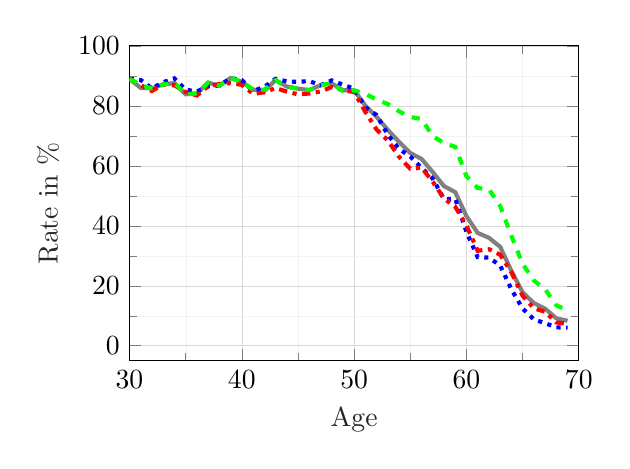
\begin{tikzpicture}
\begin{axis}[%
width=5.706cm,
height=4cm,
at={(0cm,0cm)},
scale only axis,
xmin=30,
xmax=70,
xlabel style={font=\color{white!15!black}},
xlabel={Age},
ymin=-5,
ytick={0,20,...,100},
ymax=0100,
ylabel style={font=\color{white!15!black}},
ylabel={Rate in \%},
axis background/.style={fill=white},
%title style={font=\bfseries},
title={},
legend style={at={(axis cs:30,20)}, anchor=west, legend cell align=left, align=left, draw=white!15!black, font=\scriptsize},
grid=both,
grid style={line width=0.2pt, draw=gray!30},
minor grid style={line width=0.1pt, draw=gray!10},
minor tick num=1
]
% Back line (Overall) - full
\addplot [color=gray, line width=1.5pt]
  table[row sep=crcr]{%
30	88.970588	\\
31	85.964912	\\
32	85.840708	\\
33	87.121212	\\
34	87.596899	\\
35	83.846154	\\
36	84.10596	\\
37	87.730061	\\
38	86.666667	\\
39	89.265537	\\
40	88.020833	\\
41	85.388128	\\
42	84.931507	\\
43	88.546256	\\
44	86.440678	\\
45	85.714286	\\
46	85.227273	\\
47	86.851211	\\
48	87.5	\\
49	85.185185	\\
50	85.154062	\\
51	80.060423	\\
52	76.353276	\\
53	71.967655	\\
54	67.96875	\\
55	64.268585	\\
56	62.302483	\\
57	57.905983	\\
58	53.222453	\\
59	51.209677	\\
60	43.248532	\\
61	37.619962	\\
62	36	\\
63	33.004926	\\
64	25	\\
65	17.810458	\\
66	14.24	\\
67	12.389381	\\
68	9.145427	\\
69	8.333333	\\
};
% \addlegendentry{Model} % legend shown in row (A) only

% Red line (Poor health) - dash-dotted
\addplot [color=blue, line width=1.5pt, dotted]
  table[row sep=crcr]{%
30	88.970588	\\
31	88.596491	\\
32	85.840708	\\
33	87.878788	\\
34	89.147287	\\
35	85.384615	\\
36	84.768212	\\
37	86.503067	\\
38	86.666667	\\
39	89.265537	\\
40	88.541667	\\
41	84.931507	\\
42	86.30137	\\
43	88.986784	\\
44	88.135593	\\
45	87.969925	\\
46	88.257576	\\
47	86.851211	\\
48	88.461538	\\
49	87.037037	\\
50	85.714286	\\
51	79.456193	\\
52	76.923077	\\
53	70.350404	\\
54	65.625	\\
55	63.069544	\\
56	59.367946	\\
57	55.769231	\\
58	48.856549	\\
59	48.991935	\\
60	37.964775	\\
61	29.558541	\\
62	29.391304	\\
63	26.765189	\\
64	18.833333	\\
65	12.418301	\\
66	8.8	\\
67	7.522124	\\
68	6.146927	\\
69	6.034483	\\
};
%\addlegendentry{(D3) No Cap. Gains Tax}
% \addlegendentry{(D3)} % legend shown in row (A) only
% Blue line (Good health) - dotted
\addplot [color=red, line width=1.5pt, dashdotted]
  table[row sep=crcr]{%
30	88.970588	\\
31	86.842105	\\
32	84.955752	\\
33	87.121212	\\
34	86.821705	\\
35	84.615385	\\
36	83.443709	\\
37	86.503067	\\
38	87.272727	\\
39	87.570621	\\
40	86.979167	\\
41	84.018265	\\
42	84.474886	\\
43	85.903084	\\
44	84.745763	\\
45	83.834586	\\
46	84.090909	\\
47	84.775087	\\
48	86.217949	\\
49	85.185185	\\
50	84.593838	\\
51	77.945619	\\
52	72.079772	\\
53	68.463612	\\
54	63.020833	\\
55	58.992806	\\
56	59.367946	\\
57	54.700855	\\
58	49.064449	\\
59	46.370968	\\
60	40.117417	\\
61	31.669866	\\
62	32.173913	\\
63	30.377668	\\
64	24.5	\\
65	16.666667	\\
66	12.48	\\
67	11.356932	\\
68	7.796102	\\
69	7.327586	\\
};
%\addlegendentry{(D4) No Income Tax}
% \addlegendentry{(D4)} % legend shown in row (A) only



% Green line (Disabled) - dashed
\addplot [color=green, line width=1.5pt, dashed]
  table[row sep=crcr]{%
30	88.970588	\\
31	86.842105	\\
32	85.840708	\\
33	87.121212	\\
34	87.596899	\\
35	83.846154	\\
36	84.10596	\\
37	87.730061	\\
38	86.666667	\\
39	89.265537	\\
40	88.020833	\\
41	85.388128	\\
42	85.388128	\\
43	88.546256	\\
44	86.440678	\\
45	85.714286	\\
46	85.227273	\\
47	86.851211	\\
48	87.5	\\
49	84.876543	\\
50	85.154062	\\
51	83.987915	\\
52	82.051282	\\
53	80.592992	\\
54	78.125	\\
55	76.258993	\\
56	75.620767	\\
57	69.871795	\\
58	67.567568	\\
59	66.330645	\\
60	56.555773	\\
61	52.591171	\\
62	52.173913	\\
63	46.633826	\\
64	36.666667	\\
65	27.287582	\\
66	21.76	\\
67	18.879056	\\
68	13.493253	\\
69	11.781609	\\
};
%\addlegendentry{(D5) No Disability Benefit}
% \addlegendentry{(D5)} % legend shown in row (A) only
\end{axis}
\end{tikzpicture}} \\[0.4ex]
\multicolumn{2}{c}{\small (C) Disability}\\[0.3ex]
\scalebox{0.9}{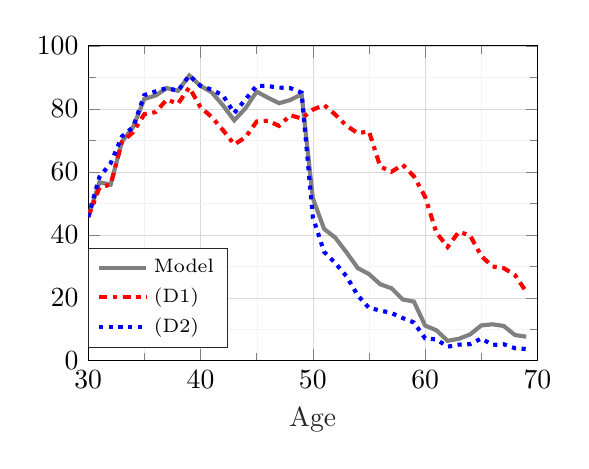
\begin{tikzpicture}
\begin{axis}[%
width=5.706cm,
height=4cm,
at={(0cm,0cm)},
scale only axis,
xmin=30,
xmax=70,
xlabel style={font=\color{white!15!black}},
xlabel={Age},
ymin=-0,
ymax=0100,
ylabel style={font=\color{white!15!black}},
ylabel={},
axis background/.style={fill=white},
%title style={font=\bfseries},
title={},
legend style={at={(axis cs:30,20)}, anchor=west, legend cell align=left, align=left, draw=white!15!black, font=\scriptsize},
grid=both,
grid style={line width=0.2pt, draw=gray!30},
minor grid style={line width=0.1pt, draw=gray!10},
minor tick num=1
]
% Back line (Overall) - full
\addplot [color=gray, line width=1.5pt]
  table[row sep=crcr]{%
30	45.652174	\\
31	56.666667	\\
32	55.932203	\\
33	69.491525	\\
34	74.193548	\\
35	83.13253	\\
36	84.210526	\\
37	86.585366	\\
38	85.714286	\\
39	90.566038	\\
40	87.288136	\\
41	85.217391	\\
42	81.102362	\\
43	76.335878	\\
44	80.141844	\\
45	85.443038	\\
46	83.536585	\\
47	81.767956	\\
48	82.795699	\\
49	84.615385	\\
50	51.612903	\\
51	41.880342	\\
52	39.08046	\\
53	34.42029	\\
54	29.431438	\\
55	27.516779	\\
56	24.28115	\\
57	23.030303	\\
58	19.469027	\\
59	18.78453	\\
60	11.167513	\\
61	9.68523	\\
62	6.338028	\\
63	6.976744	\\
64	8.351648	\\
65	11.226611	\\
66	11.583012	\\
67	11.048689	\\
68	8.166969	\\
69	7.651246	\\
};
\addlegendentry{Model}
% Blue line (Good health) - dotted
\addplot [color=red, line width=1.5pt, dashdotted]
  table[row sep=crcr]{%
30	45.652174	\\
31	55	\\
32	55.932203	\\
33	69.491525	\\
34	72.580645	\\
35	78.313253	\\
36	78.947368	\\
37	82.926829	\\
38	81.632653	\\
39	86.792453	\\
40	80.508475	\\
41	77.391304	\\
42	73.228346	\\
43	68.70229	\\
44	70.921986	\\
45	75.949367	\\
46	76.219512	\\
47	74.585635	\\
48	77.956989	\\
49	76.923077	\\
50	79.723502	\\
51	81.196581	\\
52	78.16092	\\
53	74.637681	\\
54	72.240803	\\
55	72.818792	\\
56	61.661342	\\
57	60	\\
58	62.241888	\\
59	58.563536	\\
60	52.030457	\\
61	40.677966	\\
62	36.150235	\\
63	40.930233	\\
64	39.78022	\\
65	33.264033	\\
66	29.92278	\\
67	29.400749	\\
68	27.22323	\\
69	21.886121	\\
};
%\addlegendentry{(D1) No Social Security}
\addlegendentry{(D1)}

% Red line (Poor health) - dash-dotted
\addplot [color=blue, line width=1.5pt, dotted]
  table[row sep=crcr]{%
30	45.652174	\\
31	58.333333	\\
32	62.711864	\\
33	71.186441	\\
34	74.193548	\\
35	84.337349	\\
36	85.526316	\\
37	86.585366	\\
38	85.714286	\\
39	90.566038	\\
40	87.288136	\\
41	86.086957	\\
42	84.251969	\\
43	78.625954	\\
44	82.978723	\\
45	87.341772	\\
46	87.195122	\\
47	86.740331	\\
48	86.55914	\\
49	85.128205	\\
50	45.62212	\\
51	34.615385	\\
52	31.034483	\\
53	26.811594	\\
54	20.735786	\\
55	16.778523	\\
56	15.974441	\\
57	15.151515	\\
58	13.569322	\\
59	12.154696	\\
60	7.106599	\\
61	6.779661	\\
62	4.460094	\\
63	5.116279	\\
64	5.274725	\\
65	7.068607	\\
66	5.019305	\\
67	5.243446	\\
68	3.99274	\\
69	3.736655	\\
};
%\addlegendentry{(D2) Full Medicare Ins.}
\addlegendentry{(D2)}

% Green line (Disabled) - dashed
% \addplot [color=green, line width=1.5pt, dashed]
%   table[row sep=crcr]{%
% 30	45.65217391	\\
% 31	61.66666667	\\
% 32	62.71186441	\\
% 33	71.18644068	\\
% 34	74.19354839	\\
% 35	84.3373494	\\
% 36	85.52631579	\\
% 37	86.58536585	\\
% 38	85.71428571	\\
% 39	90.56603774	\\
% 40	87.28813559	\\
% 41	86.08695652	\\
% 42	84.2519685	\\
% 43	78.6259542	\\
% 44	82.9787234	\\
% 45	87.34177215	\\
% 46	86.58536585	\\
% 47	85.63535912	\\
% 48	86.02150538	\\
% 49	85.64102564	\\
% 50	46.08294931	\\
% 51	35.47008547	\\
% 52	30.651341	\\
% 53	27.53623188	\\
% 54	23.07692308	\\
% 55	19.46308725	\\
% 56	17.25239617	\\
% 57	16.06060606	\\
% 58	13.86430678	\\
% 59	13.5359116	\\
% 60	7.614213198	\\
% 61	7.263922518	\\
% 62	4.460093897	\\
% 63	6.046511628	\\
% 64	4.835164835	\\
% 65	1.03950104	\\
% 66	0.193050193	\\
% 67	0.374531835	\\
% 68	0.362976407	\\
% 69	0.177935943	\\
% };
% \addlegendentry{Medicare B Reform Full}
\end{axis}
\end{tikzpicture}} & \scalebox{0.9}{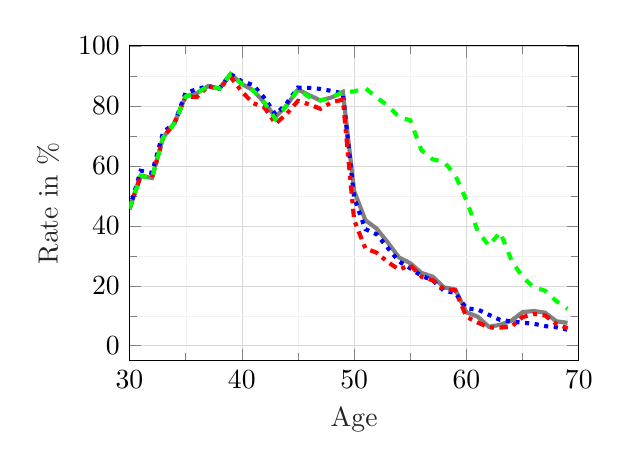
\begin{tikzpicture}
\begin{axis}[%
width=5.706cm,
height=4cm,
at={(0cm,0cm)},
scale only axis,
xmin=30,
xmax=70,
xlabel style={font=\color{white!15!black}},
xlabel={Age},
ymin=-5,
ytick={0,20,...,100},
ymax=0100,
ylabel style={font=\color{white!15!black}},
ylabel={Rate in \%},
axis background/.style={fill=white},
%title style={font=\bfseries},
title={},
legend style={at={(axis cs:30,20)}, anchor=west, legend cell align=left, align=left, draw=white!15!black, font=\scriptsize},
grid=both,
grid style={line width=0.2pt, draw=gray!30},
minor grid style={line width=0.1pt, draw=gray!10},
minor tick num=1
]
% Back line (Overall) - full
\addplot [color=gray, line width=1.5pt]
  table[row sep=crcr]{%
30	45.652174	\\
31	56.666667	\\
32	55.932203	\\
33	69.491525	\\
34	74.193548	\\
35	83.13253	\\
36	84.210526	\\
37	86.585366	\\
38	85.714286	\\
39	90.566038	\\
40	87.288136	\\
41	85.217391	\\
42	81.102362	\\
43	76.335878	\\
44	80.141844	\\
45	85.443038	\\
46	83.536585	\\
47	81.767956	\\
48	82.795699	\\
49	84.615385	\\
50	51.612903	\\
51	41.880342	\\
52	39.08046	\\
53	34.42029	\\
54	29.431438	\\
55	27.516779	\\
56	24.28115	\\
57	23.030303	\\
58	19.469027	\\
59	18.78453	\\
60	11.167513	\\
61	9.68523	\\
62	6.338028	\\
63	6.976744	\\
64	8.351648	\\
65	11.226611	\\
66	11.583012	\\
67	11.048689	\\
68	8.166969	\\
69	7.651246	\\
};
% \addlegendentry{Model} % legend shown in row (A) only

% Red line (Poor health) - dash-dotted
\addplot [color=blue, line width=1.5pt, dotted]
  table[row sep=crcr]{%
30	45.652174	\\
31	58.333333	\\
32	57.627119	\\
33	71.186441	\\
34	74.193548	\\
35	84.337349	\\
36	85.526316	\\
37	86.585366	\\
38	85.714286	\\
39	90.566038	\\
40	88.135593	\\
41	86.956522	\\
42	82.677165	\\
43	77.099237	\\
44	80.851064	\\
45	86.075949	\\
46	85.97561	\\
47	85.635359	\\
48	84.946237	\\
49	84.102564	\\
50	49.308756	\\
51	38.888889	\\
52	37.164751	\\
53	32.608696	\\
54	28.093645	\\
55	25.838926	\\
56	23.322684	\\
57	21.818182	\\
58	18.289086	\\
59	17.679558	\\
60	12.436548	\\
61	12.106538	\\
62	10.328638	\\
63	8.604651	\\
64	8.131868	\\
65	7.692308	\\
66	7.335907	\\
67	6.554307	\\
68	6.170599	\\
69	5.338078	\\
};
%\addlegendentry{(D3) No Cap. Gains Tax}
% \addlegendentry{(D3)} % legend shown in row (A) only
% Blue line (Good health) - dotted
\addplot [color=red, line width=1.5pt, dashdotted]
  table[row sep=crcr]{%
30	45.652174	\\
31	56.666667	\\
32	55.932203	\\
33	69.491525	\\
34	74.193548	\\
35	83.13253	\\
36	82.894737	\\
37	86.585366	\\
38	85.714286	\\
39	89.622642	\\
40	84.745763	\\
41	80.869565	\\
42	79.527559	\\
43	74.045802	\\
44	77.304965	\\
45	81.64557	\\
46	80.487805	\\
47	79.005525	\\
48	81.182796	\\
49	82.051282	\\
50	41.935484	\\
51	32.478632	\\
52	31.034483	\\
53	27.898551	\\
54	25.41806	\\
55	26.845638	\\
56	23.003195	\\
57	21.818182	\\
58	18.879056	\\
59	18.508287	\\
60	9.64467	\\
61	7.748184	\\
62	6.103286	\\
63	6.046512	\\
64	6.373626	\\
65	9.56341	\\
66	10.617761	\\
67	10.11236	\\
68	7.259528	\\
69	5.871886	\\
};
%\addlegendentry{(D4) No Income Tax}
% \addlegendentry{(D4)} % legend shown in row (A) only


% Green line (Disabled) - dashed
\addplot [color=green, line width=1.5pt, dashed]
  table[row sep=crcr]{%
30	45.652174	\\
31	56.666667	\\
32	55.932203	\\
33	69.491525	\\
34	74.193548	\\
35	83.13253	\\
36	84.210526	\\
37	86.585366	\\
38	85.714286	\\
39	90.566038	\\
40	87.288136	\\
41	85.217391	\\
42	81.102362	\\
43	75.572519	\\
44	80.141844	\\
45	85.443038	\\
46	82.926829	\\
47	81.767956	\\
48	82.795699	\\
49	84.615385	\\
50	84.792627	\\
51	85.897436	\\
52	82.758621	\\
53	80.072464	\\
54	76.254181	\\
55	75.167785	\\
56	65.175719	\\
57	62.121212	\\
58	61.356932	\\
59	56.906077	\\
60	48.477157	\\
61	38.256659	\\
62	33.333333	\\
63	37.906977	\\
64	28.571429	\\
65	22.869023	\\
66	19.498069	\\
67	18.35206	\\
68	14.882033	\\
69	12.27758	\\
};
%\addlegendentry{(D5) No Disability Benefit}
% \addlegendentry{(D5)} % legend shown in row (A) only
\end{axis}
\end{tikzpicture}}
\end{tabular}
\tabnotes{\textit{Notes:} Labor force participation rate (percent) by age and health status, simulated from the estimated model (Model) and from counterfactual economies that eliminate one policy instrument. Rows (A), (B), and (C) show individuals in good health, in poor health, and with a disability. Left panels: D1 sets Social Security benefits to zero; D2 sets out-of-pocket medical expenses after age 65 to zero for participants and nonparticipants. Right panels: D3 sets the net return on assets equal to the pretax return; D4 sets the income tax to zero; D5 sets disability benefits to zero. Line styles are the same in every row; the legends of row (A) identify them.}
\end{figure}
